\documentclass[tikz,border=8pt]{standalone}
% Shared look for every TikZ diagram. Load with \input{../../tools/tikz-style.tex}
\usepackage[T1]{fontenc}
\usepackage{lmodern}
\renewcommand{\sfdefault}{lmr}  % diagrams use the same serif as the text
\usetikzlibrary{arrows.meta, positioning, shapes.geometric, calc, fit, backgrounds}
\definecolor{cblue}{HTML}{4C78A8}
\definecolor{corange}{HTML}{F58518}
\definecolor{cgreen}{HTML}{54A24B}
\definecolor{cred}{HTML}{E45756}
\definecolor{cpurple}{HTML}{B279A2}
\definecolor{cgrey}{HTML}{6B6B6B}
\tikzset{
  every picture/.style={font=\sffamily, line width=1.2pt},
  box/.style={draw=#1, fill=#1!12, rounded corners=4pt, align=center, inner sep=7pt, minimum height=1.1cm},
  box/.default=cgrey,
  arrow/.style={-{Stealth[length=3mm]}, draw=cgrey, line width=1.4pt},
  title/.style={font=\sffamily\bfseries\Large},
  note/.style={font=\sffamily\small, text=cgrey, align=center},
}
\AtBeginDocument{\hyphenpenalty=10000 \exhyphenpenalty=10000}

\begin{document}
\begin{tikzpicture}[every node/.append style={font=\sffamily\Large}]
  \foreach \k in {1,...,6} {
    \ifnum\k=3 \def\c{cblue}\else\ifnum\k=6 \def\c{corange}\else\def\c{cgrey}\fi\fi
    \node[draw=\c, fill=\c!15, rounded corners=4pt, minimum size=1.3cm, line width=1.4pt] (f\k) at (1.7*\k,0) {\k};
  }
  \node[text=cblue, font=\sffamily\large\bfseries] at (f3.north) [above=3pt] {$A$};
  \node[text=corange, font=\sffamily\large\bfseries] at (f6.north) [above=3pt] {$B$};
  \node[title] at (6,2.0) {one roll of one die};
  \node[align=center, font=\sffamily\large] at (6,-1.9) {no face is in both: $P(A \cap B) = 0$};
  \node[align=center, font=\sffamily\large] at (6,-2.8) {given $B$, only face 6 is left: $P(A \mid B) = 0$};
  \node[align=center, font=\sffamily\large] at (6,-3.7) {$A$ or $B$: 2 of 6 faces, $\tfrac{1}{6} + \tfrac{1}{6} = \tfrac{1}{3}$};
\end{tikzpicture}
\end{document}
